\section{Introduction}

Let $C:=\{c_1,c_2, \ldots c_n\}$ be a set of curves for which we want 
to compute all intersections. We want to avoid testing pairs of curves 
that are far apart. To find the intersecting pairs we imagine sweeping  
a line $l$ from left to right over the plane, starting from a position 
left to all curves. While we sweep the plane, we keep track of all 
curves intersecting it.

This type of algorithm is called a {\em plane sweep algorithm} and the line 
$l$ is called the {\em sweep line}. The {\em status} of the sweep line is 
the set of curves intersecting it. The status changes while the sweep line 
moves to the right, but not continuously. The sweep line status is updated at 
specific points called the {\em event points}. These points are actually
the endpoints of all curves and their intersection points. The initial set of 
{\em event points} are only the endpoints of the curves. More
{\em event points} are added as intersection points are calculated.

This chapter describes the \ccc{Sweep_line_2} class it implements the
{\em plane sweep algorithm}, and can be used to compute the
intersection points of a given collection curves, the disjoint-interior
subcurves induced by such a collection, and a few other retaled tasks.

In particular, we take advantage of the implemented sweep line algorithm to
construct a Planar Map of intersecting curves efficiently. See 
\ccc{CGAL::Pm_with_intersection} for more deatils.

\subsection{Functionality}
Given a collection $C$ of possibly intersecting (not necessarily
$x$-monotone~\footnote{We stress this fact, because some implementation,
such as, \ccc{Planar_map_2<Dcel,Traits>} assume all curves are $x$-monotone 
in order to gain simplicity and speed.}) curves in a plane, the
\ccStyle{Sweep_line_2} class provides the following operations that can be
performed on $C$:

\begin{itemize}
\item calculate the intersection points between the curves of $C$. 
\item calculate the interior-disjoint curves induced by $C$.
\item calculate the intersection points and return a list of curves 
  participating at each intersection point.
\item answer the query whether an intersection point between any two curves
  exists.
\end{itemize}

\subsection{A Simple Program}
The simple program listed below computes all sub segments induced by 
a set of four input segments illustrated in figure \ref{SL_sec:simple}.
The endpoints of the resulting sub segments are printed out.

\begin{figure}[hbp]
\begin{ccTexOnly}
\centerline{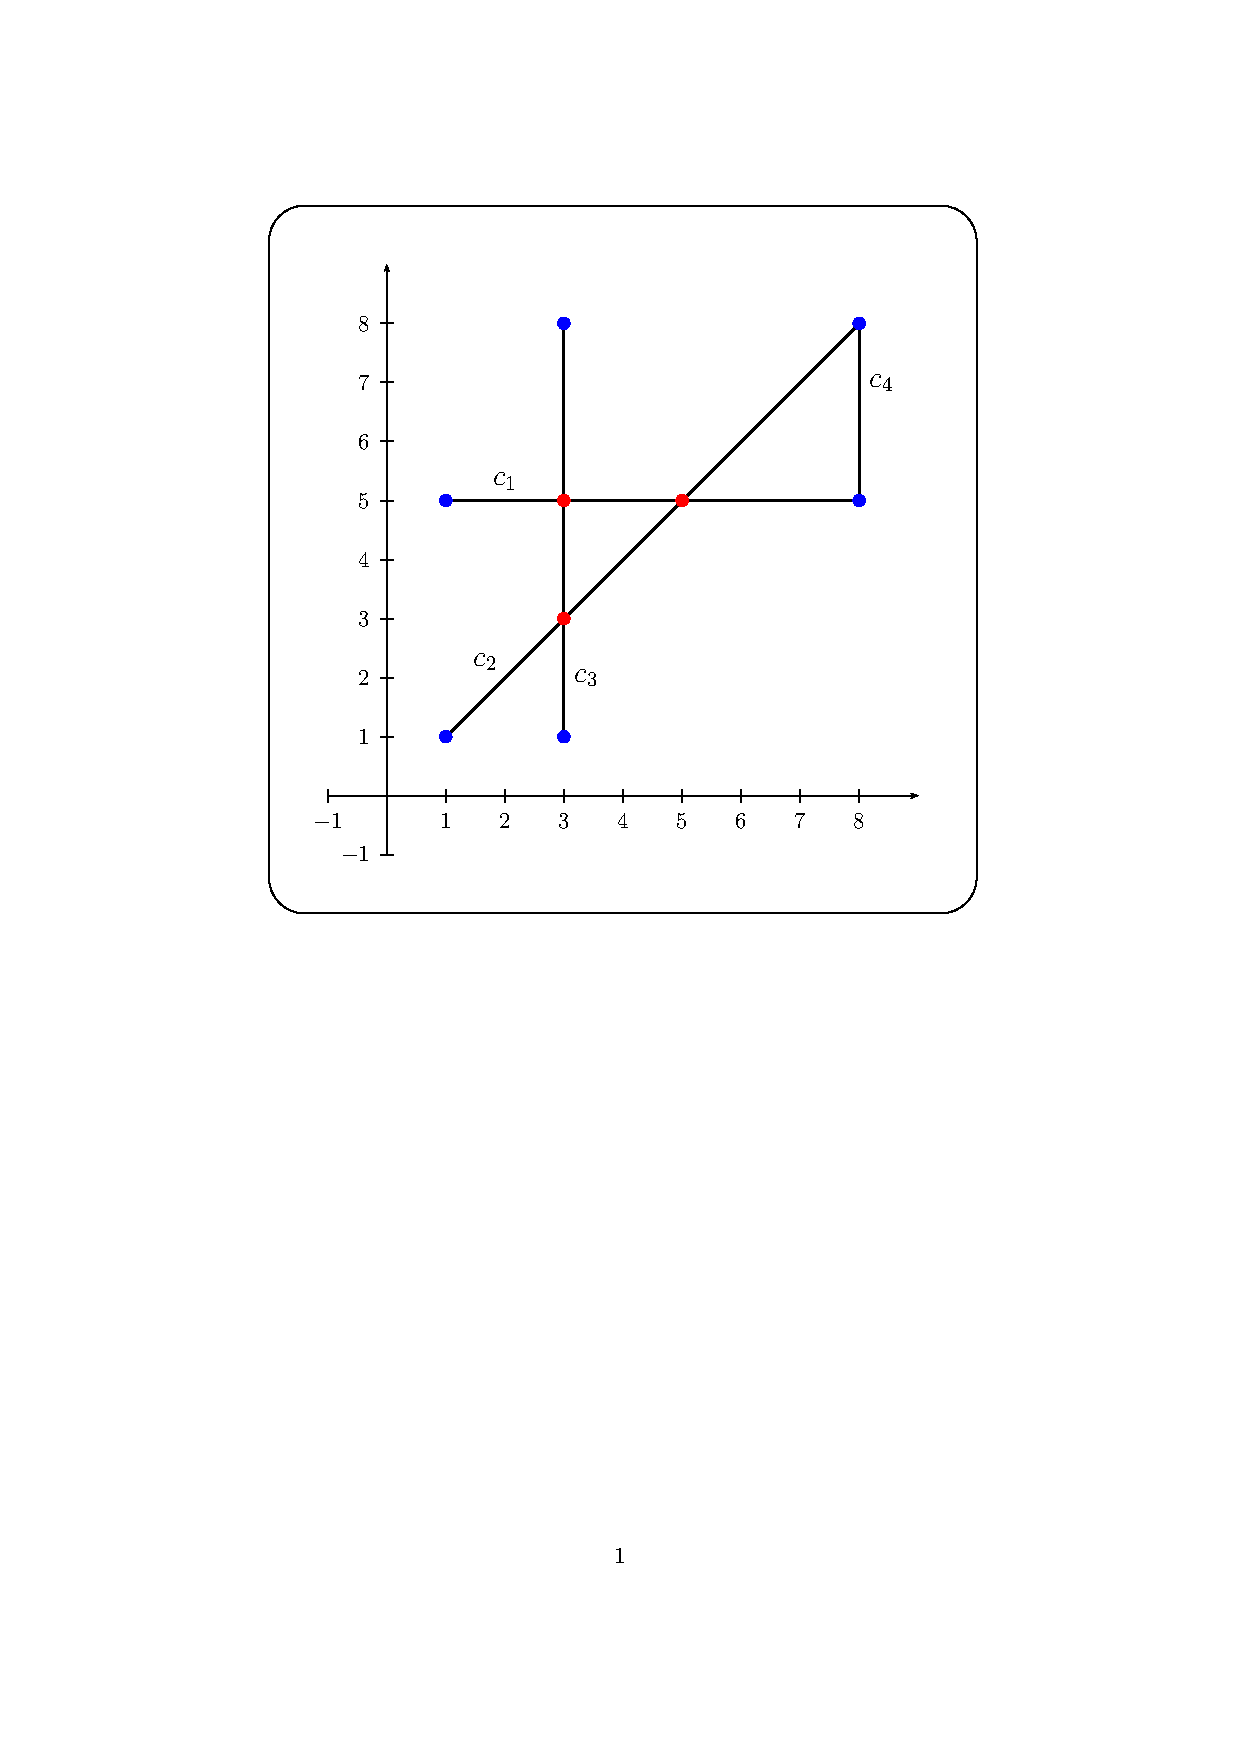
\includegraphics{Sweep_line_2/sl_simple}}
\end{ccTexOnly}

\caption{Four input segments
\label{SL_sec:simple}}

\begin{ccHtmlOnly}
<P>
<center>
  <img src="sl_simple.gif" border=0 alt="Four Input Segments">
</center>
\end{ccHtmlOnly}
\end{figure}

\begin{alltt}
#include <CGAL/Cartesian.h>
#include <CGAL/MP_Float.h>
#include <CGAL/Quotient.h>
#include <CGAL/Arr_segment_cached_traits_2.h>
#include <CGAL/Sweep_line_2.h>
#include <vector>

typedef CGAL::Quotient<CGAL::MP_Float>                  NT;
typedef CGAL::Cartesian<NT>                             Kernel;
typedef CGAL::Arr_segment_cached_traits_2<Kernel>       Traits;
typedef Traits::Point_2                                 Point_2;
typedef Traits::Curve_2                                 Curve_2;
typedef std::list<Curve_2>                              CurveList;
typedef CurveList::iterator                             CurveListIter;
typedef CGAL::Sweep_line_2<CurveListIter, Traits>       Sweep_line;

int main()
\{
  CurveList  segments;
  Curve_2 c1(Point_2(1,5), Point_2(8,5));
  Curve_2 c2(Point_2(1,1), Point_2(8,8));
  Curve_2 c3(Point_2(3,1), Point_2(3,8));
  Curve_2 c4(Point_2(8,5), Point_2(8,8));

  segments.push_back(c1);
  segments.push_back(c2);
  segments.push_back(c3);
  segments.push_back(c4);

  std::list<Curve_2> subcurves;
  Sweep_line sl;
  sl.get_subcurves(segments.begin(), segments.end(), 
		   std::back_inserter(subcurves), true);
  
  for (std::list<Curve_2>::iterator scv_iter = subcurves.begin(); 
       scv_iter != subcurves.end(); scv_iter++)
    std::cout << *scv_iter << std::endl;
  return 0;
\}
\end{alltt}

The input segments intersect at three interior points and meet at two
endpoints. The program results with ten sub segments.
The output of the program follows:

\begin{alltt}
1/1 1/1 -147/-49 -147/-49
1/1 5/1 -147/-49 -245/-49
3/1 1/1 -147/-49 -147/-49
-147/-49 -147/-49 -147/-49 -245/-49
-147/-49 -245/-49 3/1 8/1
-147/-49 -147/-49 245/49 245/49
-147/-49 -245/-49 245/49 245/49
245/49 245/49 8/1 5/1
245/49 245/49 8/1 8/1
8/1 5/1 8/1 8/1
\end{alltt}
